%!TEX root = ../Thesis.tex

\section{Recurent Neural Network}

The Skip-gram model can be interpreted as a Feedforward Network. This class of neural networks have the shortcoming that the require a fixed input size and can only look a fixed amount of steps back and forward in history. This can be a problem when analyzing sentences, because amount of words in a sentence isn't fixed and there isn't a well defined window size for the surrounding words.

The Recurrent Neural Networks (RNN) overcome this shortcoming by having an internal state. In principal this allows the network to take a sequence of vectors and consider the entire history. The sequence can be of any size, but each vector must be of the same size. In the case of sentences a fixed sized vectors is not an issue when considering a fixed vocabulary.

In practice it turns out that the RNN forgets the past and only have a short memory. Another model called Long-Short-Term-Memory (LSTM) extends the RNN and have been shown to have better performance \cite{missing source}. The ideas are however still the same, thus to understand the LSTM model a basic understanding of the RNN model is necessary.

\subsection{Forward pass}

\begin{figure}[h]
	\centering
	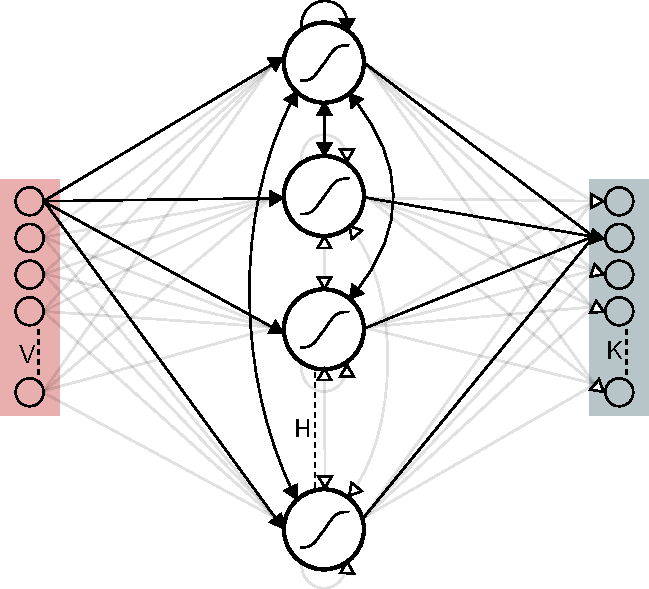
\includegraphics[scale=0.7]{theory/rnn-singlelayer-folded}
	\caption{Visualization of a single interation in a Recurent Neural Network.}
	\label{fig:theory:rnn:rnn-singlelayer-folded}
\end{figure}

Consider Figure \ref{fig:theory:rnn:rnn-singlelayer-folded} but without the extra internal connections, such that it is just a feedforward network. The elements in the input vector is then denoted $x_{i}, i \in [1, V]$, the corresponding input for the hidden layer is $a_{h}, h \in [1, H]$ with an activation $b_{h}, h \in [1, H]$. Finally there is the network output $a_{k}, k \in [1, K]$.

However since a sequence of $\mathbf{x}$ vectors will be used later, a $t \in [1, T]$ is added to the notation. Note that just because a $t$ is used, the RNN model generalizes to non-time dependent datasets as well. In the case of semantic analysis the sequence $\{\mathbf{x}^t\}_{t=1}^T$ will refer to a sequence of words represented using 1-of-V encoding. The total sequence then contains a complete sentences or paragraph. 

Now recall that in a feedforward network the input for the hidden layer is:
\begin{equation}
a_h^t = \sum_{i=1}^I w_{i h} x_i^t
\end{equation}

In the case of a RNN the input for the hidden layer ($a_h^t$) is expanded such that i depends on the hidden activation for the previous time iteration ($b_h^{t-1}$):
\begin{equation}
a_h^t = \sum_{i=1}^I w_{i h} x_i^t + \sum_{h'=1}^H w_{h' h} b_{h'}^{t-1}
\end{equation}

Thus the complete set of equations are:
\begin{equationbox}[H]
\begin{equation*}
\begin{aligned}
\text{output: } a_k^t &= \sum_{h=1}^H w_{h k} b_h^t \\
\text{hidden activation: } b_h^t &= \theta(a_h^t) \\
\text{hidden input: } a_h^t &= \sum_{i=1}^I w_{i h} x_i^t + \sum_{h'=1}^H w_{h' h} b_{h'}^{t-1}
\end{aligned}
\end{equation*}
\caption{Forward equations for a single layer RNN. $\theta$ is the activation function for the hidden layer and $b_{h'}^{0}$ is usually set to $0$.}
\end{equationbox}

\subsection{Backward pass}

While it is doable to just write out the full likelihood function and differentiate with respect to the parameters $w_{i h}$, $w_{h' h}$ and $w_{h k}$, a method similar to backpropagation can be used. The method is called backpropagation through time BPTT and is almost identical to backpropagation in the feedforward network, except that it also goes backward though time ($t$) or in this case the sequence of words.

Consider the log-likelihood function for a multiclass problem, where the probabilities $y_k$ are calculated using a softmax:
\begin{equation}
\begin{aligned}
\mathcal{L} &= - \sum_{k=1}^K z_k \ln(y_k) \\
y_k &= \frac{\mathrm{exp}(a_k)} {\sum_{k'=1}^K \mathrm{exp}(a_k')}
\end{aligned}
\end{equation}

Backpropagation makes repeated use of the chain rule to finally find the gradient with respect to the weight. First the derivative of $\mathcal{L}$ with respect to $y_k$ is found:
\begin{equation}
\frac{\partial \mathcal{L}}{\partial y_k^t} = - \sum_{k'=1}^K \frac{\partial}{\partial y_k^t} z_{k'} \ln(y_{k'}) = - \frac{z_k}{y_k}
\end{equation}

Note how the sum disappears, because there is only one case where the $y_{k'}$ within the sum, matches the $y_k$ which $\mathcal{L}$ is differentiated with respect to.
\todo{Maybe show: $\frac{\partial y_{k'}^t}{\partial a_k^t}$. Document $\delta_{k k'}$}
\begin{equation}
\begin{aligned}
\frac{\partial \mathcal{L}}{\partial a_k^t} &= \sum_{k'=1}^K \frac{\partial \mathcal{L}}{\partial y_{k'}^t} \frac{\partial y_{k'}^t}{\partial a_k^t} = \sum_{k'=1}^K \left(- \frac{z_{k'}}{y_{k'}}\right) \left( y_k \delta_{k k'} - y_k y_{k'} \right) \\
&= y_k \left( - \sum_{k'=1}^K \frac{z_{k'}}{y_{k'}}\delta_{k k'} + \sum_{k'=1}^K y_{k'} \right) = y_k \left( - \frac{z_k}{y_k} + 1 \right) \\
&= - z_k + y_k
\end{aligned}
\end{equation}

Now define:
\begin{equation}
\delta_j^t \defeq \frac{\partial \mathcal{L}}{\partial a_j^t}
\end{equation}

\todo{Check this chain rule step is correct}
\begin{equation}
\begin{aligned}
\delta_h^t &= \frac{\partial \mathcal{L}}{\partial a_h^t} = \frac{\partial \mathcal{L}}{\partial b_h^t} \frac{\partial b_h^t}{\partial a_h^t} = \frac{\partial b_h^t}{\partial a_h^t} \left( \sum_{k=1}^K \frac{\partial \mathcal{L}}{\partial a_k^t} \frac{\partial a_k^t}{\partial b_h^t} + \sum_{h'=1}^H \frac{\partial \mathcal{L}}{\partial a_{h'}^{t+1}} \frac{\partial a_{h'}^{t+1}}{\partial b_h^t} \right) \\
&= \theta(a_h^t) \left( \sum_{k=1}^K \delta_k^t w_{h k} + \sum_{h'=1}^H \delta_{h'}^{t+1} w_{h h'}\right)
\end{aligned}
\end{equation}

This can be calculated by iterating from $t = T$ to $t = 1$. For the first iteration ($t = T$) it will be necessary to define $\delta_{h}^{T+1} = 0, \forall h \in [1, H]$.

\todo{Not sure why there is no $j$ sum}
\begin{equation}
\frac{\partial \mathcal{L}}{\partial w_{ij}} = \sum_{t=1}^T \frac{\partial \mathcal{L}}{\partial a_j^t} \frac{\partial a_j^t}{\partial w_{ij}} = \sum_{t=1}^T \delta_j^t b_i^t
\end{equation}
